\documentclass[12pt, a4paper]{article}
\usepackage[dutch]{babel}
\usepackage{graphicx}
\usepackage{fullpage}
\usepackage{fancyhdr}
\usepackage{setspace}
\usepackage{color}
\usepackage{float}
\usepackage[parfill]{parskip}
\usepackage{epstopdf}
\usepackage{tabularx}
\usepackage{ctable}
\doublespacing
\pagestyle{fancyplain} {
	\fancyhead[L,R]{\thepage}
	\fancyhead[R,L]{Titouan Vervack}
}

\pagestyle{fancy}
\fancyhead{} % clear all header fields
\renewcommand{\headrulewidth}{0pt} % no line in header area
\fancyfoot{} % clear all footer fields
\fancyhead[LE,R]{\thepage}
\fancyhead[RE,L]{Titouan Vervack}
\setlength{\headsep}{15pt}

\begin{document}
\title{Programming Languages \\ Assignments}
\author{Titouan Vervack\\ Bachelor of Science in Informatics}
\date{19 May 2014}
\maketitle
\newpage
\section*{Used hardware and software}
All of the tests ran on the same hardware and software, which you can see below:\\
\textbf{Hardware:}
\begin{itemize}
	\item \textbf{CPU:} Intel I7 2600k quad core @3.4Ghz
	\item \textbf{RAM:} Corsair Vengeance 8GB (2x4GB) CL9 @1600Mhz
	\item \textbf{HDD:} Western Digital Blue 1TB 7200RPM 64MB cache\\
\end{itemize}
\textbf{Software:}
\begin{itemize}
	\item \textbf{OS:} Windows 8.1 Pro 64-bit
	\item \textbf{Compiler:} Mozart 1.4.0
\end{itemize}

Every program is a standalone program that was compiled using the command \textbf{ozc -x Code.oz}.
\section*{Assignment 1 Lazy execution}
\subsection*{Assignment 1.1 Performance isssues}
For this assignment I decided to implement the Sieve of Eratosthenes and the mergesort algorithm. The sieve commands expect one integer as input which represents the upperbound for the sieve. Mergesort expects one integer as input which represents the amount of numbers to sort. Mergesort first creates a list of N random elements in Oz and then sorts it.
\subsection*{Sieve of Eratosthenes}
In the lazy version everything is lazy, including the parsing of the input arguments. The eager version on the other hand does nothing lazily. The eager and lazy version are almost exactly the same. The only difference are the lazy keywords in front of every function and an added touch function, to force the list of prime numbers to be calculated.\\
Since both versions are so alike their time complexity is the same. We observe that the lazy version is slower though. Lazy evaluation should be preferred if it allows us to skip the calculation of certain parts in the program. This also means that when the same amount of information has to be calculated, lazy does worse than eager since it has more overhead. This is lazy evaluation's drawback. In the case of this Sieve, both lazy and eager have to calculate the same amount of information. This makes the eager version more preferable since it is as easy to write as the lazy version and performs better (less overhead).

We can see the results of the benchmark beneath.
\begin{center}
% GNUPLOT: LaTeX picture with Postscript
\begingroup
  \makeatletter
  \providecommand\color[2][]{%
    \GenericError{(gnuplot) \space\space\space\@spaces}{%
      Package color not loaded in conjunction with
      terminal option `colourtext'%
    }{See the gnuplot documentation for explanation.%
    }{Either use 'blacktext' in gnuplot or load the package
      color.sty in LaTeX.}%
    \renewcommand\color[2][]{}%
  }%
  \providecommand\includegraphics[2][]{%
    \GenericError{(gnuplot) \space\space\space\@spaces}{%
      Package graphicx or graphics not loaded%
    }{See the gnuplot documentation for explanation.%
    }{The gnuplot epslatex terminal needs graphicx.sty or graphics.sty.}%
    \renewcommand\includegraphics[2][]{}%
  }%
  \providecommand\rotatebox[2]{#2}%
  \@ifundefined{ifGPcolor}{%
    \newif\ifGPcolor
    \GPcolorfalse
  }{}%
  \@ifundefined{ifGPblacktext}{%
    \newif\ifGPblacktext
    \GPblacktexttrue
  }{}%
  % define a \g@addto@macro without @ in the name:
  \let\gplgaddtomacro\g@addto@macro
  % define empty templates for all commands taking text:
  \gdef\gplbacktext{}%
  \gdef\gplfronttext{}%
  \makeatother
  \ifGPblacktext
    % no textcolor at all
    \def\colorrgb#1{}%
    \def\colorgray#1{}%
  \else
    % gray or color?
    \ifGPcolor
      \def\colorrgb#1{\color[rgb]{#1}}%
      \def\colorgray#1{\color[gray]{#1}}%
      \expandafter\def\csname LTw\endcsname{\color{white}}%
      \expandafter\def\csname LTb\endcsname{\color{black}}%
      \expandafter\def\csname LTa\endcsname{\color{black}}%
      \expandafter\def\csname LT0\endcsname{\color[rgb]{1,0,0}}%
      \expandafter\def\csname LT1\endcsname{\color[rgb]{0,1,0}}%
      \expandafter\def\csname LT2\endcsname{\color[rgb]{0,0,1}}%
      \expandafter\def\csname LT3\endcsname{\color[rgb]{1,0,1}}%
      \expandafter\def\csname LT4\endcsname{\color[rgb]{0,1,1}}%
      \expandafter\def\csname LT5\endcsname{\color[rgb]{1,1,0}}%
      \expandafter\def\csname LT6\endcsname{\color[rgb]{0,0,0}}%
      \expandafter\def\csname LT7\endcsname{\color[rgb]{1,0.3,0}}%
      \expandafter\def\csname LT8\endcsname{\color[rgb]{0.5,0.5,0.5}}%
    \else
      % gray
      \def\colorrgb#1{\color{black}}%
      \def\colorgray#1{\color[gray]{#1}}%
      \expandafter\def\csname LTw\endcsname{\color{white}}%
      \expandafter\def\csname LTb\endcsname{\color{black}}%
      \expandafter\def\csname LTa\endcsname{\color{black}}%
      \expandafter\def\csname LT0\endcsname{\color{black}}%
      \expandafter\def\csname LT1\endcsname{\color{black}}%
      \expandafter\def\csname LT2\endcsname{\color{black}}%
      \expandafter\def\csname LT3\endcsname{\color{black}}%
      \expandafter\def\csname LT4\endcsname{\color{black}}%
      \expandafter\def\csname LT5\endcsname{\color{black}}%
      \expandafter\def\csname LT6\endcsname{\color{black}}%
      \expandafter\def\csname LT7\endcsname{\color{black}}%
      \expandafter\def\csname LT8\endcsname{\color{black}}%
    \fi
  \fi
  \setlength{\unitlength}{0.0500bp}%
  \begin{picture}(7200.00,5040.00)%
    \gplgaddtomacro\gplbacktext{%
      \csname LTb\endcsname%
      \put(1210,704){\makebox(0,0)[r]{\strut{} 0}}%
      \csname LTb\endcsname%
      \put(1210,1111){\makebox(0,0)[r]{\strut{} 2000}}%
      \csname LTb\endcsname%
      \put(1210,1518){\makebox(0,0)[r]{\strut{} 4000}}%
      \csname LTb\endcsname%
      \put(1210,1925){\makebox(0,0)[r]{\strut{} 6000}}%
      \csname LTb\endcsname%
      \put(1210,2332){\makebox(0,0)[r]{\strut{} 8000}}%
      \csname LTb\endcsname%
      \put(1210,2740){\makebox(0,0)[r]{\strut{} 10000}}%
      \csname LTb\endcsname%
      \put(1210,3147){\makebox(0,0)[r]{\strut{} 12000}}%
      \csname LTb\endcsname%
      \put(1210,3554){\makebox(0,0)[r]{\strut{} 14000}}%
      \csname LTb\endcsname%
      \put(1210,3961){\makebox(0,0)[r]{\strut{} 16000}}%
      \csname LTb\endcsname%
      \put(1210,4368){\makebox(0,0)[r]{\strut{} 18000}}%
      \csname LTb\endcsname%
      \put(1210,4775){\makebox(0,0)[r]{\strut{} 20000}}%
      \csname LTb\endcsname%
      \put(1342,484){\makebox(0,0){\strut{} 100}}%
      \csname LTb\endcsname%
      \put(1949,484){\makebox(0,0){\strut{} 200}}%
      \csname LTb\endcsname%
      \put(2556,484){\makebox(0,0){\strut{} 300}}%
      \csname LTb\endcsname%
      \put(3162,484){\makebox(0,0){\strut{} 400}}%
      \csname LTb\endcsname%
      \put(3769,484){\makebox(0,0){\strut{} 500}}%
      \csname LTb\endcsname%
      \put(4376,484){\makebox(0,0){\strut{} 600}}%
      \csname LTb\endcsname%
      \put(4983,484){\makebox(0,0){\strut{} 700}}%
      \csname LTb\endcsname%
      \put(5589,484){\makebox(0,0){\strut{} 800}}%
      \csname LTb\endcsname%
      \put(6196,484){\makebox(0,0){\strut{} 900}}%
      \csname LTb\endcsname%
      \put(6803,484){\makebox(0,0){\strut{} 1000}}%
      \put(176,2739){\rotatebox{-270}{\makebox(0,0){\strut{}Processing time (ms)}}}%
      \put(4072,154){\makebox(0,0){\strut{}Input size (in thousands)}}%
    }%
    \gplgaddtomacro\gplfronttext{%
      \csname LTb\endcsname%
      \put(2134,4602){\makebox(0,0)[r]{\strut{}Eager}}%
      \csname LTb\endcsname%
      \put(2134,4382){\makebox(0,0)[r]{\strut{}Lazy}}%
    }%
    \gplbacktext
    \put(0,0){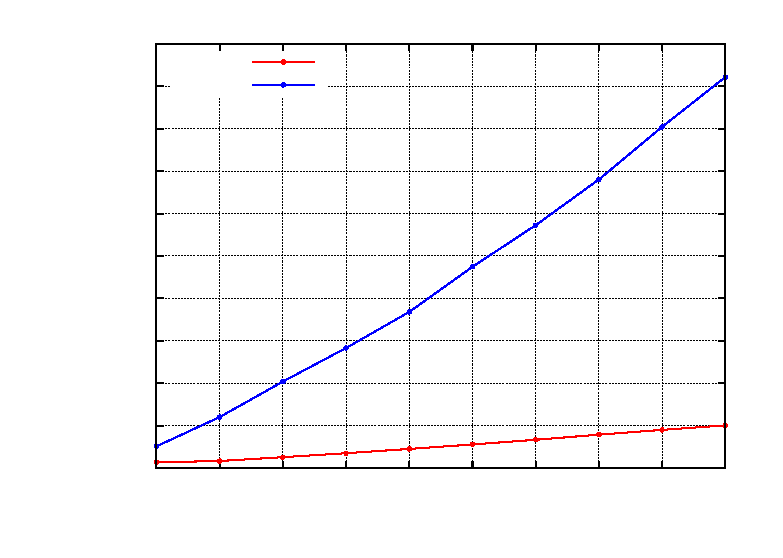
\includegraphics{Sieve}}%
    \gplfronttext
  \end{picture}%
\endgroup

\end{center}
We ran the test 10 times over each the lazy and the eager version. The input parameter varied between $100.000$ en $1.000.000$ and was incremented in steps of $100.000$. The batch script that was used to benchmark the programs can be found in \textbf{Assignment 1.1/SieveTester.bat}. The data can be found in \textbf{EagerSieve.dat} and \textbf{LazySieve.dat}.
\subsection*{Mergesort}
The lazy and eager version both contain a procedure(Split). As it is a procedure this is always eager. Every function in the lazy version is again lazy and there is an extra touch function as in the Sieve exercise. Because of this the time complexity of both versions is the same, but the lazy is slower because of the introduced overhead. So again, the eager version is preferred.

We can see the results of the benchmark beneath.
\begin{center}
% GNUPLOT: LaTeX picture with Postscript
\begingroup
  \makeatletter
  \providecommand\color[2][]{%
    \GenericError{(gnuplot) \space\space\space\@spaces}{%
      Package color not loaded in conjunction with
      terminal option `colourtext'%
    }{See the gnuplot documentation for explanation.%
    }{Either use 'blacktext' in gnuplot or load the package
      color.sty in LaTeX.}%
    \renewcommand\color[2][]{}%
  }%
  \providecommand\includegraphics[2][]{%
    \GenericError{(gnuplot) \space\space\space\@spaces}{%
      Package graphicx or graphics not loaded%
    }{See the gnuplot documentation for explanation.%
    }{The gnuplot epslatex terminal needs graphicx.sty or graphics.sty.}%
    \renewcommand\includegraphics[2][]{}%
  }%
  \providecommand\rotatebox[2]{#2}%
  \@ifundefined{ifGPcolor}{%
    \newif\ifGPcolor
    \GPcolorfalse
  }{}%
  \@ifundefined{ifGPblacktext}{%
    \newif\ifGPblacktext
    \GPblacktexttrue
  }{}%
  % define a \g@addto@macro without @ in the name:
  \let\gplgaddtomacro\g@addto@macro
  % define empty templates for all commands taking text:
  \gdef\gplbacktext{}%
  \gdef\gplfronttext{}%
  \makeatother
  \ifGPblacktext
    % no textcolor at all
    \def\colorrgb#1{}%
    \def\colorgray#1{}%
  \else
    % gray or color?
    \ifGPcolor
      \def\colorrgb#1{\color[rgb]{#1}}%
      \def\colorgray#1{\color[gray]{#1}}%
      \expandafter\def\csname LTw\endcsname{\color{white}}%
      \expandafter\def\csname LTb\endcsname{\color{black}}%
      \expandafter\def\csname LTa\endcsname{\color{black}}%
      \expandafter\def\csname LT0\endcsname{\color[rgb]{1,0,0}}%
      \expandafter\def\csname LT1\endcsname{\color[rgb]{0,1,0}}%
      \expandafter\def\csname LT2\endcsname{\color[rgb]{0,0,1}}%
      \expandafter\def\csname LT3\endcsname{\color[rgb]{1,0,1}}%
      \expandafter\def\csname LT4\endcsname{\color[rgb]{0,1,1}}%
      \expandafter\def\csname LT5\endcsname{\color[rgb]{1,1,0}}%
      \expandafter\def\csname LT6\endcsname{\color[rgb]{0,0,0}}%
      \expandafter\def\csname LT7\endcsname{\color[rgb]{1,0.3,0}}%
      \expandafter\def\csname LT8\endcsname{\color[rgb]{0.5,0.5,0.5}}%
    \else
      % gray
      \def\colorrgb#1{\color{black}}%
      \def\colorgray#1{\color[gray]{#1}}%
      \expandafter\def\csname LTw\endcsname{\color{white}}%
      \expandafter\def\csname LTb\endcsname{\color{black}}%
      \expandafter\def\csname LTa\endcsname{\color{black}}%
      \expandafter\def\csname LT0\endcsname{\color{black}}%
      \expandafter\def\csname LT1\endcsname{\color{black}}%
      \expandafter\def\csname LT2\endcsname{\color{black}}%
      \expandafter\def\csname LT3\endcsname{\color{black}}%
      \expandafter\def\csname LT4\endcsname{\color{black}}%
      \expandafter\def\csname LT5\endcsname{\color{black}}%
      \expandafter\def\csname LT6\endcsname{\color{black}}%
      \expandafter\def\csname LT7\endcsname{\color{black}}%
      \expandafter\def\csname LT8\endcsname{\color{black}}%
    \fi
  \fi
  \setlength{\unitlength}{0.0500bp}%
  \begin{picture}(7200.00,5040.00)%
    \gplgaddtomacro\gplbacktext{%
      \csname LTb\endcsname%
      \put(1210,704){\makebox(0,0)[r]{\strut{} 0}}%
      \csname LTb\endcsname%
      \put(1210,1286){\makebox(0,0)[r]{\strut{} 5000}}%
      \csname LTb\endcsname%
      \put(1210,1867){\makebox(0,0)[r]{\strut{} 10000}}%
      \csname LTb\endcsname%
      \put(1210,2449){\makebox(0,0)[r]{\strut{} 15000}}%
      \csname LTb\endcsname%
      \put(1210,3030){\makebox(0,0)[r]{\strut{} 20000}}%
      \csname LTb\endcsname%
      \put(1210,3612){\makebox(0,0)[r]{\strut{} 25000}}%
      \csname LTb\endcsname%
      \put(1210,4193){\makebox(0,0)[r]{\strut{} 30000}}%
      \csname LTb\endcsname%
      \put(1210,4775){\makebox(0,0)[r]{\strut{} 35000}}%
      \csname LTb\endcsname%
      \put(1342,484){\makebox(0,0){\strut{} 100}}%
      \csname LTb\endcsname%
      \put(1949,484){\makebox(0,0){\strut{} 200}}%
      \csname LTb\endcsname%
      \put(2556,484){\makebox(0,0){\strut{} 300}}%
      \csname LTb\endcsname%
      \put(3162,484){\makebox(0,0){\strut{} 400}}%
      \csname LTb\endcsname%
      \put(3769,484){\makebox(0,0){\strut{} 500}}%
      \csname LTb\endcsname%
      \put(4376,484){\makebox(0,0){\strut{} 600}}%
      \csname LTb\endcsname%
      \put(4983,484){\makebox(0,0){\strut{} 700}}%
      \csname LTb\endcsname%
      \put(5589,484){\makebox(0,0){\strut{} 800}}%
      \csname LTb\endcsname%
      \put(6196,484){\makebox(0,0){\strut{} 900}}%
      \csname LTb\endcsname%
      \put(6803,484){\makebox(0,0){\strut{} 1000}}%
      \put(176,2739){\rotatebox{-270}{\makebox(0,0){\strut{}Processing time (ms)}}}%
      \put(4072,154){\makebox(0,0){\strut{}Input size (in thousands)}}%
    }%
    \gplgaddtomacro\gplfronttext{%
      \csname LTb\endcsname%
      \put(2134,4602){\makebox(0,0)[r]{\strut{}Eager}}%
      \csname LTb\endcsname%
      \put(2134,4382){\makebox(0,0)[r]{\strut{}Lazy}}%
    }%
    \gplbacktext
    \put(0,0){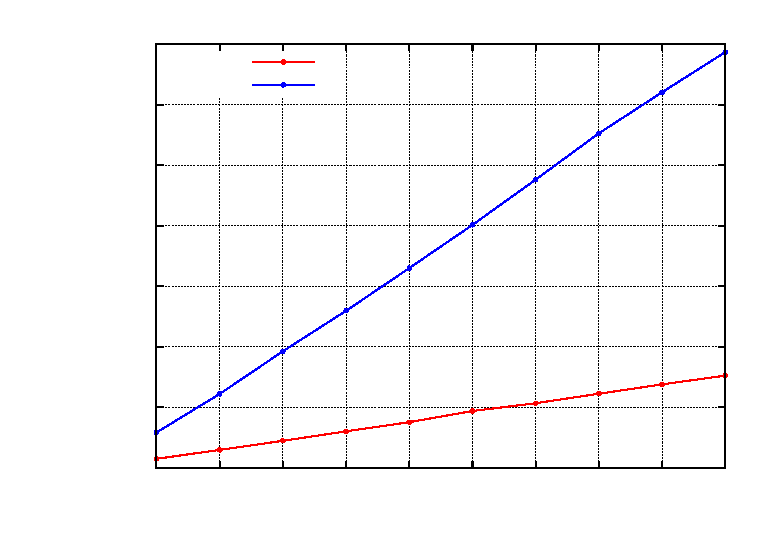
\includegraphics{Sort}}%
    \gplfronttext
  \end{picture}%
\endgroup

\end{center}
We ran the test 10 times over each the lazy and the eager version. The input parameter varied between $100.000$ en $1.000.000$ and was incremented in steps of $100.000$. The batch script that was used to benchmark the programs can be found in \textbf{Assignment 1.1/SortTester.bat}. The data can be found in \textbf{EagerSort.dat} and \textbf{LazySort.dat}.
\subsection*{Assignment 1.2 The Hamming problem}
The lazy version is a more general version of the Hamming problem which is solved in the book (page 293-294). This solution makes use of an infinite stream H. An eager version for this problem can't use an infinite list which forces us to adjust the algorithm. This is why eager and lazy aren't completely comparable.\\
The eager version uses some lazyness. The first K prime numbers are calculated lazily (as in the lazy version) using the Sieve of Eratosthenes we wrote in the previous assignment. After that though, everything is eager. The way we solve this problem is as follows:
\begin{itemize}
\item Calculate the first K primes.
\item While we don't have N elements in H (the current resultset): loop over every prime number x in the set of K prime numbers.
\item Loop over the elements of H until you find the first element y which is bigger than the last element in H when multiplied with x. Return x * y.
\item Save these minima for every prime.
\item Calculate the minimum of these minima and add it to H. Start over from the first step until we have enough elements. 
\end{itemize}

I ran one benchmark which went over the lazy and eager version a 100 times each. We observed how changing N(the amount of numbers to generate) and K(the amount of primes to use) influenced the processing time of the program. N ranged between $10.000$ and $20.000$ (which I increased in steps of $1.000$) while K ranged between $5$ and $15$ (which I increased in steps of $1$). We used some of this data to produce the graphs below. 

\begin{center}
% GNUPLOT: LaTeX picture with Postscript
\begingroup
  \makeatletter
  \providecommand\color[2][]{%
    \GenericError{(gnuplot) \space\space\space\@spaces}{%
      Package color not loaded in conjunction with
      terminal option `colourtext'%
    }{See the gnuplot documentation for explanation.%
    }{Either use 'blacktext' in gnuplot or load the package
      color.sty in LaTeX.}%
    \renewcommand\color[2][]{}%
  }%
  \providecommand\includegraphics[2][]{%
    \GenericError{(gnuplot) \space\space\space\@spaces}{%
      Package graphicx or graphics not loaded%
    }{See the gnuplot documentation for explanation.%
    }{The gnuplot epslatex terminal needs graphicx.sty or graphics.sty.}%
    \renewcommand\includegraphics[2][]{}%
  }%
  \providecommand\rotatebox[2]{#2}%
  \@ifundefined{ifGPcolor}{%
    \newif\ifGPcolor
    \GPcolorfalse
  }{}%
  \@ifundefined{ifGPblacktext}{%
    \newif\ifGPblacktext
    \GPblacktexttrue
  }{}%
  % define a \g@addto@macro without @ in the name:
  \let\gplgaddtomacro\g@addto@macro
  % define empty templates for all commands taking text:
  \gdef\gplbacktext{}%
  \gdef\gplfronttext{}%
  \makeatother
  \ifGPblacktext
    % no textcolor at all
    \def\colorrgb#1{}%
    \def\colorgray#1{}%
  \else
    % gray or color?
    \ifGPcolor
      \def\colorrgb#1{\color[rgb]{#1}}%
      \def\colorgray#1{\color[gray]{#1}}%
      \expandafter\def\csname LTw\endcsname{\color{white}}%
      \expandafter\def\csname LTb\endcsname{\color{black}}%
      \expandafter\def\csname LTa\endcsname{\color{black}}%
      \expandafter\def\csname LT0\endcsname{\color[rgb]{1,0,0}}%
      \expandafter\def\csname LT1\endcsname{\color[rgb]{0,1,0}}%
      \expandafter\def\csname LT2\endcsname{\color[rgb]{0,0,1}}%
      \expandafter\def\csname LT3\endcsname{\color[rgb]{1,0,1}}%
      \expandafter\def\csname LT4\endcsname{\color[rgb]{0,1,1}}%
      \expandafter\def\csname LT5\endcsname{\color[rgb]{1,1,0}}%
      \expandafter\def\csname LT6\endcsname{\color[rgb]{0,0,0}}%
      \expandafter\def\csname LT7\endcsname{\color[rgb]{1,0.3,0}}%
      \expandafter\def\csname LT8\endcsname{\color[rgb]{0.5,0.5,0.5}}%
    \else
      % gray
      \def\colorrgb#1{\color{black}}%
      \def\colorgray#1{\color[gray]{#1}}%
      \expandafter\def\csname LTw\endcsname{\color{white}}%
      \expandafter\def\csname LTb\endcsname{\color{black}}%
      \expandafter\def\csname LTa\endcsname{\color{black}}%
      \expandafter\def\csname LT0\endcsname{\color{black}}%
      \expandafter\def\csname LT1\endcsname{\color{black}}%
      \expandafter\def\csname LT2\endcsname{\color{black}}%
      \expandafter\def\csname LT3\endcsname{\color{black}}%
      \expandafter\def\csname LT4\endcsname{\color{black}}%
      \expandafter\def\csname LT5\endcsname{\color{black}}%
      \expandafter\def\csname LT6\endcsname{\color{black}}%
      \expandafter\def\csname LT7\endcsname{\color{black}}%
      \expandafter\def\csname LT8\endcsname{\color{black}}%
    \fi
  \fi
  \setlength{\unitlength}{0.0500bp}%
  \begin{picture}(7200.00,5040.00)%
    \gplgaddtomacro\gplbacktext{%
      \csname LTb\endcsname%
      \put(1210,704){\makebox(0,0)[r]{\strut{} 0}}%
      \csname LTb\endcsname%
      \put(1210,1229){\makebox(0,0)[r]{\strut{} 10000}}%
      \csname LTb\endcsname%
      \put(1210,1754){\makebox(0,0)[r]{\strut{} 20000}}%
      \csname LTb\endcsname%
      \put(1210,2279){\makebox(0,0)[r]{\strut{} 30000}}%
      \csname LTb\endcsname%
      \put(1210,2804){\makebox(0,0)[r]{\strut{} 40000}}%
      \csname LTb\endcsname%
      \put(1210,3329){\makebox(0,0)[r]{\strut{} 50000}}%
      \csname LTb\endcsname%
      \put(1210,3854){\makebox(0,0)[r]{\strut{} 60000}}%
      \csname LTb\endcsname%
      \put(1210,4379){\makebox(0,0)[r]{\strut{} 70000}}%
      \csname LTb\endcsname%
      \put(1342,484){\makebox(0,0){\strut{} 10}}%
      \csname LTb\endcsname%
      \put(2434,484){\makebox(0,0){\strut{} 12}}%
      \csname LTb\endcsname%
      \put(3526,484){\makebox(0,0){\strut{} 14}}%
      \csname LTb\endcsname%
      \put(4619,484){\makebox(0,0){\strut{} 16}}%
      \csname LTb\endcsname%
      \put(5711,484){\makebox(0,0){\strut{} 18}}%
      \csname LTb\endcsname%
      \put(6803,484){\makebox(0,0){\strut{} 20}}%
      \put(176,2541){\rotatebox{-270}{\makebox(0,0){\strut{}Processing time (ms)}}}%
      \put(4072,154){\makebox(0,0){\strut{}Numbers to generate (in thousands)}}%
      \put(4072,4709){\makebox(0,0){\strut{}K=5}}%
    }%
    \gplgaddtomacro\gplfronttext{%
      \csname LTb\endcsname%
      \put(2134,4206){\makebox(0,0)[r]{\strut{}Eager}}%
      \csname LTb\endcsname%
      \put(2134,3986){\makebox(0,0)[r]{\strut{}Lazy}}%
    }%
    \gplbacktext
    \put(0,0){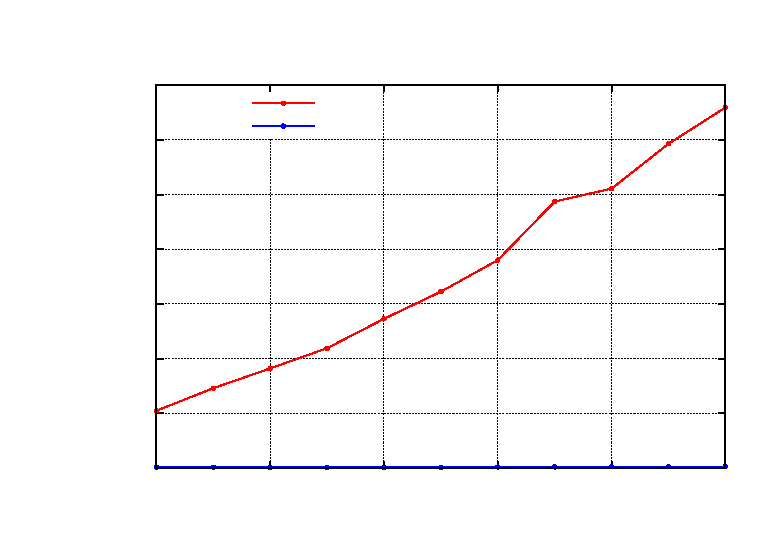
\includegraphics{HammingN}}%
    \gplfronttext
  \end{picture}%
\endgroup

\end{center}
For this graph we let N vary between $10.000$ and $20.000$ while K held the constant value $5$.
\begin{center}
% GNUPLOT: LaTeX picture with Postscript
\begingroup
  \makeatletter
  \providecommand\color[2][]{%
    \GenericError{(gnuplot) \space\space\space\@spaces}{%
      Package color not loaded in conjunction with
      terminal option `colourtext'%
    }{See the gnuplot documentation for explanation.%
    }{Either use 'blacktext' in gnuplot or load the package
      color.sty in LaTeX.}%
    \renewcommand\color[2][]{}%
  }%
  \providecommand\includegraphics[2][]{%
    \GenericError{(gnuplot) \space\space\space\@spaces}{%
      Package graphicx or graphics not loaded%
    }{See the gnuplot documentation for explanation.%
    }{The gnuplot epslatex terminal needs graphicx.sty or graphics.sty.}%
    \renewcommand\includegraphics[2][]{}%
  }%
  \providecommand\rotatebox[2]{#2}%
  \@ifundefined{ifGPcolor}{%
    \newif\ifGPcolor
    \GPcolorfalse
  }{}%
  \@ifundefined{ifGPblacktext}{%
    \newif\ifGPblacktext
    \GPblacktexttrue
  }{}%
  % define a \g@addto@macro without @ in the name:
  \let\gplgaddtomacro\g@addto@macro
  % define empty templates for all commands taking text:
  \gdef\gplbacktext{}%
  \gdef\gplfronttext{}%
  \makeatother
  \ifGPblacktext
    % no textcolor at all
    \def\colorrgb#1{}%
    \def\colorgray#1{}%
  \else
    % gray or color?
    \ifGPcolor
      \def\colorrgb#1{\color[rgb]{#1}}%
      \def\colorgray#1{\color[gray]{#1}}%
      \expandafter\def\csname LTw\endcsname{\color{white}}%
      \expandafter\def\csname LTb\endcsname{\color{black}}%
      \expandafter\def\csname LTa\endcsname{\color{black}}%
      \expandafter\def\csname LT0\endcsname{\color[rgb]{1,0,0}}%
      \expandafter\def\csname LT1\endcsname{\color[rgb]{0,1,0}}%
      \expandafter\def\csname LT2\endcsname{\color[rgb]{0,0,1}}%
      \expandafter\def\csname LT3\endcsname{\color[rgb]{1,0,1}}%
      \expandafter\def\csname LT4\endcsname{\color[rgb]{0,1,1}}%
      \expandafter\def\csname LT5\endcsname{\color[rgb]{1,1,0}}%
      \expandafter\def\csname LT6\endcsname{\color[rgb]{0,0,0}}%
      \expandafter\def\csname LT7\endcsname{\color[rgb]{1,0.3,0}}%
      \expandafter\def\csname LT8\endcsname{\color[rgb]{0.5,0.5,0.5}}%
    \else
      % gray
      \def\colorrgb#1{\color{black}}%
      \def\colorgray#1{\color[gray]{#1}}%
      \expandafter\def\csname LTw\endcsname{\color{white}}%
      \expandafter\def\csname LTb\endcsname{\color{black}}%
      \expandafter\def\csname LTa\endcsname{\color{black}}%
      \expandafter\def\csname LT0\endcsname{\color{black}}%
      \expandafter\def\csname LT1\endcsname{\color{black}}%
      \expandafter\def\csname LT2\endcsname{\color{black}}%
      \expandafter\def\csname LT3\endcsname{\color{black}}%
      \expandafter\def\csname LT4\endcsname{\color{black}}%
      \expandafter\def\csname LT5\endcsname{\color{black}}%
      \expandafter\def\csname LT6\endcsname{\color{black}}%
      \expandafter\def\csname LT7\endcsname{\color{black}}%
      \expandafter\def\csname LT8\endcsname{\color{black}}%
    \fi
  \fi
  \setlength{\unitlength}{0.0500bp}%
  \begin{picture}(7200.00,5040.00)%
    \gplgaddtomacro\gplbacktext{%
      \csname LTb\endcsname%
      \put(1210,704){\makebox(0,0)[r]{\strut{} 0}}%
      \csname LTb\endcsname%
      \put(1210,1072){\makebox(0,0)[r]{\strut{} 1000}}%
      \csname LTb\endcsname%
      \put(1210,1439){\makebox(0,0)[r]{\strut{} 2000}}%
      \csname LTb\endcsname%
      \put(1210,1807){\makebox(0,0)[r]{\strut{} 3000}}%
      \csname LTb\endcsname%
      \put(1210,2174){\makebox(0,0)[r]{\strut{} 4000}}%
      \csname LTb\endcsname%
      \put(1210,2542){\makebox(0,0)[r]{\strut{} 5000}}%
      \csname LTb\endcsname%
      \put(1210,2909){\makebox(0,0)[r]{\strut{} 6000}}%
      \csname LTb\endcsname%
      \put(1210,3277){\makebox(0,0)[r]{\strut{} 7000}}%
      \csname LTb\endcsname%
      \put(1210,3644){\makebox(0,0)[r]{\strut{} 8000}}%
      \csname LTb\endcsname%
      \put(1210,4012){\makebox(0,0)[r]{\strut{} 9000}}%
      \csname LTb\endcsname%
      \put(1210,4379){\makebox(0,0)[r]{\strut{} 10000}}%
      \csname LTb\endcsname%
      \put(1888,484){\makebox(0,0){\strut{} 6}}%
      \csname LTb\endcsname%
      \put(2980,484){\makebox(0,0){\strut{} 8}}%
      \csname LTb\endcsname%
      \put(4073,484){\makebox(0,0){\strut{} 10}}%
      \csname LTb\endcsname%
      \put(5165,484){\makebox(0,0){\strut{} 12}}%
      \csname LTb\endcsname%
      \put(6257,484){\makebox(0,0){\strut{} 14}}%
      \put(176,2541){\rotatebox{-270}{\makebox(0,0){\strut{}Processing time (ms)}}}%
      \put(4072,154){\makebox(0,0){\strut{}Amount of primes}}%
      \put(4072,4709){\makebox(0,0){\strut{}N=10.000}}%
    }%
    \gplgaddtomacro\gplfronttext{%
      \csname LTb\endcsname%
      \put(5816,4206){\makebox(0,0)[r]{\strut{}Eager}}%
      \csname LTb\endcsname%
      \put(5816,3986){\makebox(0,0)[r]{\strut{}Lazy}}%
    }%
    \gplbacktext
    \put(0,0){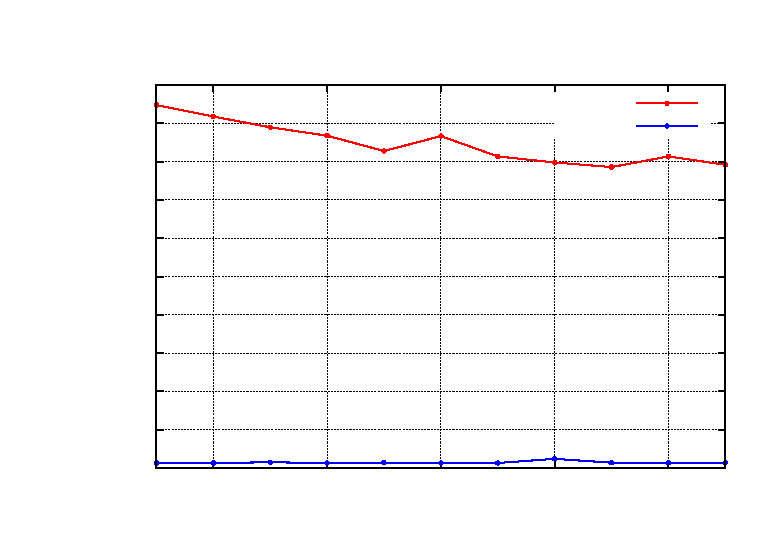
\includegraphics{HammingK}}%
    \gplfronttext
  \end{picture}%
\endgroup

\end{center}
For this graph we let K vary between $5$ and $15$ while N held the constant value $10.000$.

We see that eager version is always a lot slower. This is because it isn't able to make use of the optimized algorithm. We can also observe that the processing time gets reduced when we use more prime numbers.

We can conclude that the lazy version is a lot faster (because it can make use of the infinite stream) and is easier to write. Because of this the lazy version is preferred over the eager version.
The lazy version is able to complete the task in $O(N)$ time. The eager version on the other hand does it in $O(N * (K * log(N)))$.

The batch script that was used to benchmark the programs can be found in \textbf{Assignment 1.1/HammingTester.bat}. The data can be found in the folder \textbf{Assignment 1.2} in the files \textbf{EagerHamming.dat} and \textbf{LazyHamming.dat}. The data for the graphs can be found in the same folder in the files \textbf{LazyHammingCstN.dat}, \textbf{LazyHammingCstK.dat}, \textbf{EagerHammingCstN.dat} and \textbf{EagerHammingCstK.dat}
\section*{Assignment 2 Declarative model and concurrency}
For this assignment I turned the sudokus into csv's. Every cage gets appointed a character. For each element in the sudoku I write down the right character and a comma. This creates a file of 81 characters seperated by comma's, representing the sudoku. After the sudoku I write down the character of every cage and it's number, again seperated by commas. You end up with one very long, comma seperated line which can be used to let the programs solve the sudoku.

You can find these Sudoku files in \textbf{Assignment 2.1/Sudoku.csv}, \textbf{Assignment 2.2/Sudoku1.csv} and \textbf{Assignment 2.2/Sudoku2.csv}.
\subsection*{Assignment 2.1 Declarative model}
This program was written in Oz. The way I solved this was by using Oz' constraints. Using this makes it quite easy to solve the KillerSudoku. We first parse the csv into a 9x9 matrix containing the sudoku and then parse the values of the cages and save those in a list of tuples. After parsing, we create a new 9x9 matrix using \textbf{FD.list}. We add the regular sudoku constraints. The first of these constraints is that the numbers in a sudoku varie between 1-9. The second is that no two numbers in the same row,column or box have the same value. For this we use \textbf{FD.distinct}. The only thing that's different about a KillerSudoku is that it has cages. So we add a constraint for these cages. We use \textbf{FD.sum} in combination with the Sudoku matrix and the list of sum tuples to pull this off.

The solution is actually found within a fraction of a second but for completeness we did a test. This test can be found in \textbf{Assignment 2.2/KillerSudokuTester.bat}. After running the test we know that the solution is computed within 50 ms.\\
The solution we found is the folowing:\\
\begin{center}
\begin{tabularx}{6.03cm}{!{\vrule width 2pt}c|c|c!{\vrule width 2pt}c|c|c!{\vrule width 2pt}c|c|c!{\vrule width 2pt}}
\specialrule{.2em}{0em}{0em}
5&8&1&3&4&2&9&7&6\\
\hline
4&3&6&5&7&9&8&1&2\\
\hline
7&9&2&8&6&1&4&5&3\\
\specialrule{.2em}{0em}{0em}
6&4&5&7&1&3&2&8&9\\
\hline
3&7&9&4&2&8&1&6&5\\
\hline
2&1&8&6&9&5&3&4&7\\
\specialrule{.2em}{0em}{0em}
8&6&4&2&3&7&5&9&1\\
\hline
9&5&3&1&8&6&7&2&4\\
\hline
1&2&7&9&5&4&6&3&8\\
\specialrule{.2em}{0em}{0em}
\end{tabularx}
\end{center}
We are able to conclude that using constraints in Oz was the right choice for this problem. It was not too hard to implement and is very fast (50ms). Writing this in a language like Java would have taken a lot longer as it would've probably needed backtracking.
\subsection*{Assignment 2.2 Introducing concurrency}
The concurrent model we used was the declarative concurrent model. The reason I chose this model is because it is easy to implement. The other models would have been a lot more work to implement and I don't think they would've have made the computation any faster.\\

The program runs two searches, each in it's seperate thread, and makes use of the dataflow variable \textbf{Sol} to communicate between these threads. Unification of the threads is done by the barrier defined in the book on page 277.\\

Sadly, I was unable to produce a solution using my concurrent program. I am also unable to conclude if this is because of a programming error or just because the problem takes too long to solve.\\
Even though my concurrent program didn't work, I was able to find the solution to the linked sudoku killer by using the program of the previous assignment. The solution I found is the following:\\
\begin{center}
\begin{tabularx}{6.03cm}{!{\vrule width 2pt}c|c|c!{\vrule width 2pt}c|c|c!{\vrule width 2pt}c|c|c!{\vrule width 2pt}}
\specialrule{.2em}{0em}{0em}
6&5&8&7&2&1&3&4&9\\
\hline
3&9&1&4&5&6&7&8&2\\
\hline
4&7&2&3&8&9&5&6&1\\
\specialrule{.2em}{0em}{0em}
2&6&4&5&9&3&1&7&8\\
\hline
1&3&7&6&4&8&9&2&5\\
\hline
5&8&9&1&7&2&4&3&6\\
\specialrule{.2em}{0em}{0em}
7&2&3&8&1&5&6&9&4\\
\hline
8&1&6&9&3&4&2&5&7\\
\hline
9&4&5&2&6&7&8&1&3\\
\specialrule{.2em}{0em}{0em}
\end{tabularx}
\end{center}
\end{document}